% !TeX root = RJwrapper.tex
\title{The \texttt{doBy} package -- yet another utility package}
\author{by Søren Højsgaard}

\maketitle

\abstract{%
The \texttt{doBy} is one of several general utility packages on CRAN. We
illustrate two main features of the package: The ability to making
groupwise computations and the ability to compute linear estimates,
contrasts and least-squares means.
}

\hypertarget{introduction}{%
\subsection{Introduction}\label{introduction}}

The package originally grew out of a need to calculate groupwise summary
statistics (much in the spirit of \texttt{PROC\ SUMMARY} of the
\texttt{SAS} system, \citep{procsummary}). The name \texttt{doBy} comes
from the need to \textbf{do} some computations on data which is
stratified \textbf{By} the value of some variables. The \texttt{doBy}
package \citep{doby} appeared on CRAN in 2006. Today the package
contains many additional utilities.

When it comes to data handling, \texttt{doBy} is nowhere nearly as
powerful as more contemporary packages, such as those in the
\texttt{tidyverse} eco system, \citep{tidyverse}. On the other hand,
\texttt{doBy} is based on classical data structures that are unlikely to
undergo sudden changes. Moreover, it can be hypothesized that the data
handling functions in \texttt{doBy} remain appealing to a group of users
because of their simplicity in use.

In this paper we focus 1) on the ``doing by'' functions and 2) on
functions related to linear estimates and contrasts.

\hypertarget{functions-related-to-groupwise-computations}{%
\subsection{Functions related to groupwise
computations}\label{functions-related-to-groupwise-computations}}

\hypertarget{a-working-dataset---the-co2-data}{%
\subsubsection{\texorpdfstring{A working dataset - the \texttt{CO2}
data}{A working dataset - the CO2 data}}\label{a-working-dataset---the-co2-data}}

The \texttt{CO2} data frame comes from an experiment on the cold
tolerance of the grass species \emph{Echinochloa crus-galli}. To limit
the amount of output we modify names and levels of variables as follows

\begin{Schunk}
\begin{Sinput}
data(CO2)
CO2 <- within(CO2, {
    Treat <- Treatment
    Treatment <- NULL
    levels(Treat) <- c("nchil", "chil")
    levels(Type)  <- c("Que", "Mis")
})
CO2 <- subset(CO2, Plant %in% c("Qn1", "Qc1", "Mn1", "Mc1"))
dim(CO2)
\end{Sinput}
\begin{Soutput}
#> [1] 28  5
\end{Soutput}
\begin{Sinput}
head(CO2, 4)
\end{Sinput}
\begin{Soutput}
#>   Plant Type conc uptake Treat
#> 1   Qn1  Que   95   16.0 nchil
#> 2   Qn1  Que  175   30.4 nchil
#> 3   Qn1  Que  250   34.8 nchil
#> 4   Qn1  Que  350   37.2 nchil
\end{Soutput}
\end{Schunk}

\hypertarget{the-summaryby-function}{%
\subsubsection{\texorpdfstring{The \texttt{summaryBy}
function}{The summaryBy function}}\label{the-summaryby-function}}

The \texttt{summaryBy} function is used for calculating quantities like
\emph{the mean and variance of numerical variables \texttt{x} and
\texttt{y} for each combination of two factors \texttt{A} and
\texttt{B\$}}. Notice: A functionality similar to \texttt{summaryBy} is
provided by \texttt{aggregate} from base R, but \texttt{summaryBy}
offers additional features.

\begin{Schunk}
\begin{Sinput}
myfun1 <- function(x){c(m=mean(x), s=sd(x))}
summaryBy(cbind(conc, uptake, lu=log(uptake)) ~ Plant, data=CO2, FUN=myfun1)
\end{Sinput}
\begin{Soutput}
#>   Plant conc.m conc.s uptake.m uptake.s  lu.m   lu.s
#> 1   Qn1    435  317.7    33.23    8.215 3.467 0.3189
#> 2   Qc1    435  317.7    29.97    8.335 3.356 0.3446
#> 3   Mn1    435  317.7    26.40    8.694 3.209 0.4234
#> 4   Mc1    435  317.7    18.00    4.119 2.864 0.2622
\end{Soutput}
\begin{Sinput}
## same as
## aggregate(cbind(conc, uptake, log(uptake)) ~ Plant, data=CO2, FUN=myfun1)
\end{Sinput}
\end{Schunk}

The convention is that variables that do not appear in the dataframe
(e.g.~\texttt{log(uptake)}) must be named (here as \texttt{lu}). Various
shportcuts are available, e.g.~the following, where left hand side dot
refers to ``all numeric variables'' while the right hand side dot refers
to ``all factor variables''. Writing \texttt{1} on the right hand side
leads to computing over the entire dataset:

\begin{Schunk}
\begin{Sinput}
summaryBy(. ~ ., data=CO2, FUN=myfun1)
\end{Sinput}
\begin{Soutput}
#>   Plant Type Treat conc.m conc.s uptake.m uptake.s
#> 1   Qn1  Que nchil    435  317.7    33.23    8.215
#> 2   Qc1  Que  chil    435  317.7    29.97    8.335
#> 3   Mn1  Mis nchil    435  317.7    26.40    8.694
#> 4   Mc1  Mis  chil    435  317.7    18.00    4.119
\end{Soutput}
\begin{Sinput}
summaryBy(. ~ 1, data=CO2, FUN=myfun1)
\end{Sinput}
\begin{Soutput}
#>   conc.m conc.s uptake.m uptake.s
#> 1    435  299.6     26.9    9.189
\end{Soutput}
\end{Schunk}

\hypertarget{formulas-and-lists}{%
\subsubsection{Formulas and lists}\label{formulas-and-lists}}

The convention for the ``By''-functions is that a two sided formula like
can be written in two ways:

\begin{Schunk}
\begin{Sinput}
cbind(x, y) ~ A + B
list(c("x", "y"), c("A", "B"))
\end{Sinput}
\end{Schunk}

Some ``By''-functions only take a right hand sided formula as input.
Such a formula can also be written in two ways:

\begin{Schunk}
\begin{Sinput}
~ A + B
c("A", "B")
\end{Sinput}
\end{Schunk}

The list-form / vector-form is especially useful if a function is
invoked programatically. Hence the calls to \texttt{summaryBy} above can
also be made as

\begin{Schunk}
\begin{Sinput}
summaryBy(list(c("conc", "uptake", "lu=log(uptake)"), "Plant"), data=CO2, FUN=myfun1)
summaryBy(list(c("."), c(".")), data=CO2, FUN=myfun1)
summaryBy(list(c("."), c("1")), data=CO2, FUN=myfun1)
\end{Sinput}
\end{Schunk}

\hypertarget{the-orderby-function}{%
\subsubsection{\texorpdfstring{The \texttt{orderBy}
function}{The orderBy function}}\label{the-orderby-function}}

Ordering (or sorting) a data frame is possible with the \texttt{orderBy}
function. Suppose we want to order the rows of the the \texttt{CO2} data
by increasing values of \texttt{conc} and decreasing value of
\texttt{uptake} (within \texttt{conc}):

\begin{Schunk}
\begin{Sinput}
x1 <- orderBy(~ conc - uptake, data=CO2)
head(x1)
\end{Sinput}
\begin{Soutput}
#>    Plant Type conc uptake Treat
#> 1    Qn1  Que   95   16.0 nchil
#> 22   Qc1  Que   95   14.2  chil
#> 43   Mn1  Mis   95   10.6 nchil
#> 64   Mc1  Mis   95   10.5  chil
#> 2    Qn1  Que  175   30.4 nchil
#> 23   Qc1  Que  175   24.1  chil
\end{Soutput}
\end{Schunk}

Following the remarks about specification in ``By''-functions, an
equivalent form is:

\begin{Schunk}
\begin{Sinput}
orderBy(c("conc", "-uptake"), data=CO2) 
\end{Sinput}
\end{Schunk}

\hypertarget{the-splitby-function}{%
\subsubsection{\texorpdfstring{The \texttt{splitBy}
function}{The splitBy function}}\label{the-splitby-function}}

Suppose we want to split \texttt{CO2} into a list of dataframes:

\begin{Schunk}
\begin{Sinput}
x1 <- splitBy(~ Plant + Type, data=CO2)
x1
\end{Sinput}
\begin{Soutput}
#>   listentry Plant Type
#> 1   Qn1|Que   Qn1  Que
#> 2   Qc1|Que   Qc1  Que
#> 3   Mn1|Mis   Mn1  Mis
#> 4   Mc1|Mis   Mc1  Mis
\end{Soutput}
\end{Schunk}

The result is a list (with a few additional attributes):

\begin{Schunk}
\begin{Sinput}
lapply(x1, head, 2)
\end{Sinput}
\begin{Soutput}
#> $`Qn1|Que`
#>   Plant Type conc uptake Treat
#> 1   Qn1  Que   95   16.0 nchil
#> 2   Qn1  Que  175   30.4 nchil
#> 
#> $`Qc1|Que`
#>    Plant Type conc uptake Treat
#> 22   Qc1  Que   95   14.2  chil
#> 23   Qc1  Que  175   24.1  chil
#> 
#> $`Mn1|Mis`
#>    Plant Type conc uptake Treat
#> 43   Mn1  Mis   95   10.6 nchil
#> 44   Mn1  Mis  175   19.2 nchil
#> 
#> $`Mc1|Mis`
#>    Plant Type conc uptake Treat
#> 64   Mc1  Mis   95   10.5  chil
#> 65   Mc1  Mis  175   14.9  chil
\end{Soutput}
\end{Schunk}

\hypertarget{the-subsetby-function}{%
\subsubsection{\texorpdfstring{The \texttt{subsetBy}
function}{The subsetBy function}}\label{the-subsetby-function}}

Suppose we want to select those rows within each treatment for which the
uptake is larger than 75\% quantile of uptake (within the treatment).
This is achieved by:

\begin{Schunk}
\begin{Sinput}
x2 <- subsetBy(~ Treat, subset=uptake > quantile(uptake, prob=0.75), data=CO2)
head(x2, 4)
\end{Sinput}
\begin{Soutput}
#>          Plant Type conc uptake Treat
#> nchil.4    Qn1  Que  350   37.2 nchil
#> nchil.6    Qn1  Que  675   39.2 nchil
#> nchil.7    Qn1  Que 1000   39.7 nchil
#> nchil.49   Mn1  Mis 1000   35.5 nchil
\end{Soutput}
\end{Schunk}

\hypertarget{the-transformby-function}{%
\subsubsection{\texorpdfstring{The \texttt{transformBy}
function}{The transformBy function}}\label{the-transformby-function}}

The \texttt{transformBy} function is analogous to the \texttt{transform}
function except that it works within groups. For example:

\begin{Schunk}
\begin{Sinput}
x3 <- transformBy(~ Treat, data=CO2, 
                 minU=min(uptake), maxU=max(uptake),
                 range=diff(range(uptake)))
head(x3, 4)
\end{Sinput}
\begin{Soutput}
#>         Plant Type conc uptake Treat minU maxU range
#> nchil.1   Qn1  Que   95   16.0 nchil 10.6 39.7  29.1
#> nchil.2   Qn1  Que  175   30.4 nchil 10.6 39.7  29.1
#> nchil.3   Qn1  Que  250   34.8 nchil 10.6 39.7  29.1
#> nchil.4   Qn1  Que  350   37.2 nchil 10.6 39.7  29.1
\end{Soutput}
\end{Schunk}

\hypertarget{the-lmby-function}{%
\subsubsection{\texorpdfstring{The \texttt{lmBy}
function}{The lmBy function}}\label{the-lmby-function}}

The \texttt{lmBy} function allows for fitting linear models to different
strata of data (the vertical bar is used for defining groupings of
data):

\begin{Schunk}
\begin{Sinput}
m <- lmBy(uptake ~ conc | Treat, data=CO2)
coef(m)
\end{Sinput}
\begin{Soutput}
#>       (Intercept)    conc
#> nchil       20.82 0.02067
#> chil        17.02 0.01602
\end{Soutput}
\end{Schunk}

The result is a list with a few additional attributes and the list can
be processed further as e.g.

\begin{Schunk}
\begin{Sinput}
lapply(m, function(z) coef(summary(z)))
\end{Sinput}
\begin{Soutput}
#> $nchil
#>             Estimate Std. Error t value  Pr(>|t|)
#> (Intercept) 20.82342   3.092430   6.734 2.092e-05
#> conc         0.02067   0.005889   3.510 4.304e-03
#> 
#> $chil
#>             Estimate Std. Error t value  Pr(>|t|)
#> (Intercept) 17.01814   3.668315   4.639 0.0005709
#> conc         0.01602   0.006986   2.293 0.0407168
\end{Soutput}
\end{Schunk}

\hypertarget{functions-related-linear-estimates-and-contrasts}{%
\subsection{Functions related linear estimates and
contrasts}\label{functions-related-linear-estimates-and-contrasts}}

A linear function of a \(p\)--dimensional parameter vector \(\beta\) has
the form \begin{displaymath}
  C=L\beta
\end{displaymath} where \(L\) is a \(q\times p\) matrix which we call
the \texttt{Linear\ Estimate\ Matrix} or simply \texttt{LE-matrix}. The
corresponding linear estimate is \(\hat C = L \hat \beta\). A linear
hypothesis has the form \(H_0: L\beta=m\) for some \(q\) dimensional
vector \(m\).

\hypertarget{a-working-dataset---the-toothgrowth-data}{%
\subsubsection{\texorpdfstring{A working dataset - the
\texttt{ToothGrowth}
data}{A working dataset - the ToothGrowth data}}\label{a-working-dataset---the-toothgrowth-data}}

The response is the length of odontoblasts cells (cells responsible for
tooth growth) in 60 guinea pigs. Each animal received one of three dose
levels of vitamin C (0.5, 1, and 2 mg/day) by one of two delivery
methods, (orange juice (coded as OJ) or ascorbic acid (a form of vitamin
C and (coded as VC)). The dataset is balanced with 10 measurements for
each combination of \texttt{dose} and \texttt{supp}. To illustrated
certain points in what follows we make data unbalance by removing the
some rows of the dataframe:

\begin{Schunk}
\begin{Sinput}
data("ToothGrowth")
ToothGrowth <- transform(ToothGrowth, dose = factor(dose))
ToothGrowth <- ToothGrowth[-(1:3), ]
head(ToothGrowth, 4)
\end{Sinput}
\begin{Soutput}
#>    len supp dose
#> 4  5.8   VC  0.5
#> 5  6.4   VC  0.5
#> 6 10.0   VC  0.5
#> 7 11.2   VC  0.5
\end{Soutput}
\end{Schunk}

\begin{Schunk}
\begin{figure}
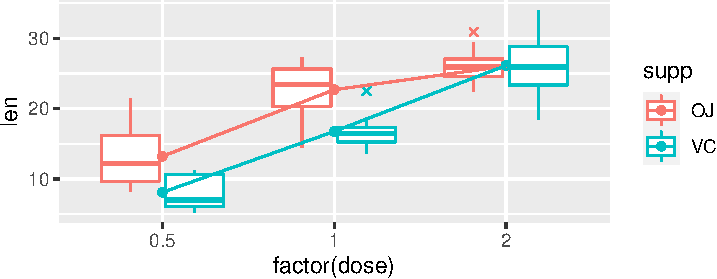
\includegraphics[keepaspectratio]{fig/doby-linear:interaction2-1} \caption[Interaction plot for the ToothGrowth data]{Interaction plot for the ToothGrowth data. The average `len` for each group is a dot. Boxplot outliers are crosses.}\label{fig:linear:interaction2}
\end{figure}
\end{Schunk}

The interaction plot indicates some interaction between \texttt{dose}
and \texttt{supp}. This is also supported by a formal test:

\begin{Schunk}
\begin{Sinput}
tooth1 <- lm(len ~ dose + supp, data=ToothGrowth)
tooth2 <- lm(len ~ dose * supp, data=ToothGrowth)
anova(tooth1, tooth2)
\end{Sinput}
\begin{Soutput}
#> Analysis of Variance Table
#> 
#> Model 1: len ~ dose + supp
#> Model 2: len ~ dose * supp
#>   Res.Df RSS Df Sum of Sq    F Pr(>F)
#> 1     53 789                         
#> 2     51 685  2       104 3.88  0.027
\end{Soutput}
\end{Schunk}

\hypertarget{computing-linear-estimates}{%
\subsubsection{Computing linear
estimates}\label{computing-linear-estimates}}

For now, we focus on the additive model. Consider computing the
estimated length for each dose of orange juice (OJ): One option:
Construct the LE--matrix \(L\) directly and then invoke \texttt{linest}:

\begin{Schunk}
\begin{Sinput}
L <- matrix(c(1, 0, 0, 0, 
              1, 1, 0, 0,
              1, 0, 1, 0), nrow=3, byrow=T)
\end{Sinput}
\end{Schunk}

The matrix \(L\) can be generated as follows:

\begin{Schunk}
\begin{Sinput}
L <- LE_matrix(tooth1, effect="dose", at=list(supp="OJ"))
\end{Sinput}
\end{Schunk}

The estimates can be computed directly as

\begin{Schunk}
\begin{Sinput}
L %*% coef(tooth1)
\end{Sinput}
\end{Schunk}

but we do not obtain standard errors etc. this way. Instead we can
invoke \texttt{linest}

\begin{Schunk}
\begin{Sinput}
c1 <- linest(tooth1, L)
coef(c1)
\end{Sinput}
\begin{Soutput}
#>   estimate std.error statistic df   p.value
#> 1    12.59     1.027     12.26 53 4.239e-17
#> 2    21.52     1.004     21.43 53 8.969e-28
#> 3    27.88     1.004     27.77 53 2.958e-33
\end{Soutput}
\begin{Sinput}
confint(c1)
\end{Sinput}
\begin{Soutput}
#>   0.025 0.975
#> 1 10.53 14.65
#> 2 19.50 23.53
#> 3 25.87 29.90
\end{Soutput}
\end{Schunk}

The function \texttt{esticon} has been part of \texttt{doBy} for many
years while \texttt{linest} is a newer addition. The functionality,
however, is similar:

\begin{Schunk}
\begin{Sinput}
c1 <- esticon(tooth1, L)
c1
\end{Sinput}
\begin{Soutput}
#>      estimate std.error statistic p.value beta0 df
#> [1,]    12.59      1.03     12.26    0.00  0.00 53
#> [2,]    21.52      1.00     21.43    0.00  0.00 53
#> [3,]    27.88      1.00     27.77    0.00  0.00 53
\end{Soutput}
\end{Schunk}

\hypertarget{least-squares-means-lsmeans}{%
\subsubsection{Least-squares means
(LS--means)}\label{least-squares-means-lsmeans}}

A related question could be: What is the estimated length for each dose
if we ignore the source of vitamin C (i.e.~whether it is OJ or VC). One
approach would be to fit a model in which source does not appear:

\begin{Schunk}
\begin{Sinput}
tooth0 <- update(tooth1, . ~ . - supp)
L0 <- LE_matrix(tooth0, effect="dose")
L0
\end{Sinput}
\begin{Soutput}
#>      (Intercept) dose1 dose2
#> [1,]           1     0     0
#> [2,]           1     1     0
#> [3,]           1     0     1
\end{Soutput}
\begin{Sinput}
linest(tooth0, L=L0)
\end{Sinput}
\begin{Soutput}
#> Coefficients:
#>      estimate std.error statistic     df p.value
#> [1,]   11.124     1.027    10.830 54.000       0
#> [2,]   19.735     0.947    20.841 54.000       0
#> [3,]   26.100     0.947    27.562 54.000       0
\end{Soutput}
\end{Schunk}

An alternative would be to stick to the original model but compute the
estimate for an ``average vitamin C source''. That would correspond to
giving weight \(1/2\) to each of the two vitamin C source parameters.
However, as one of the parameters is already set to zero to obtain
identifiability, we obtain the LE--matrix \(L\) as

\begin{Schunk}
\begin{Sinput}
L1 <- matrix(c(1, 0, 0, 0.5, 
               1, 1, 0, 0.5,
               1, 0, 1, 0.5), nrow=3, byrow=T)
linest(tooth1, L=L1)
\end{Sinput}
\begin{Soutput}
#> Coefficients:
#>      estimate std.error statistic     df p.value
#> [1,]   10.809     0.940    11.496 53.000       0
#> [2,]   19.735     0.863    22.873 53.000       0
#> [3,]   26.100     0.863    30.249 53.000       0
\end{Soutput}
\end{Schunk}

Such a particular linear estimate is sometimes called a
\emph{least-squares mean}, an \emph{LSmean}, a \emph{marginal mean} or a
\emph{population mean}. Notice: One may generate \(L\) automatically
with

\begin{Schunk}
\begin{Sinput}
L1 <- LE_matrix(tooth1, effect="dose")
L1
\end{Sinput}
\begin{Soutput}
#>      (Intercept) dose1 dose2 suppVC
#> [1,]           1     0     0    0.5
#> [2,]           1     1     0    0.5
#> [3,]           1     0     1    0.5
\end{Soutput}
\end{Schunk}

Notice: One may obtain the LSmean directly as:

\begin{Schunk}
\begin{Sinput}
LSmeans(tooth1, effect="dose")
\end{Sinput}
\begin{Soutput}
#> Coefficients:
#>      estimate std.error statistic     df p.value
#> [1,]   10.809     0.940    11.496 53.000       0
#> [2,]   19.735     0.863    22.873 53.000       0
#> [3,]   26.100     0.863    30.249 53.000       0
\end{Soutput}
\end{Schunk}

which is the same as

\begin{Schunk}
\begin{Sinput}
L <- LE_matrix(tooth1, effect="dose")
linest(tooth1, L=L)
\end{Sinput}
\end{Schunk}

\hypertarget{interaction-model}{%
\subsubsection{Interaction model}\label{interaction-model}}

For a model with interactions, the LSmeans are

\begin{Schunk}
\begin{Sinput}
LSmeans(tooth2, effect="dose")
\end{Sinput}
\begin{Soutput}
#> Coefficients:
#>      estimate std.error statistic     df p.value
#> [1,]   10.672     0.903    11.819 51.000       0
#> [2,]   19.735     0.819    24.085 51.000       0
#> [3,]   26.100     0.819    31.853 51.000       0
\end{Soutput}
\end{Schunk}

In this case, the LE--matrix is

\begin{Schunk}
\begin{Sinput}
L <- LE_matrix(tooth2, effect="dose")
L
\end{Sinput}
\begin{Soutput}
#>      (Intercept) dose1 dose2 suppVC dose1:suppVC dose2:suppVC
#> [1,]           1     0     0    0.5          0.0          0.0
#> [2,]           1     1     0    0.5          0.5          0.0
#> [3,]           1     0     1    0.5          0.0          0.5
\end{Soutput}
\end{Schunk}

\hypertarget{using-transformed-covariates}{%
\subsubsection{Using (transformed)
covariates}\label{using-transformed-covariates}}

Below, the covariate \texttt{conc} is fixed at the average value:

\begin{Schunk}
\begin{Sinput}
co2.lm1 <- lm(uptake ~ conc + Type + Treat, data=CO2)
LSmeans(co2.lm1, effect="Treat")
\end{Sinput}
\begin{Soutput}
#> Coefficients:
#>      estimate std.error statistic    df p.value
#> [1,]    29.81      1.35     22.16 24.00       0
#> [2,]    23.99      1.35     17.83 24.00       0
\end{Soutput}
\end{Schunk}

If we use \texttt{log(conc)} instead we will get an error when
calculating LS--means because \texttt{log(conc)} is not a variable in
the dataframe. Instead one can do:

\begin{Schunk}
\begin{Sinput}
co2.lm2 <- lm(uptake ~ log.conc + Type + Treat,
             data=transform(CO2, log.conc=log(conc)))
LSmeans(co2.lm2, effect="Treat")
\end{Sinput}
\begin{Soutput}
#> Coefficients:
#>      estimate std.error statistic     df p.value
#> [1,]   29.814     0.934    31.938 24.000       0
#> [2,]   23.986     0.934    25.694 24.000       0
\end{Soutput}
\end{Schunk}

This also highlights what is computed: The average of the log of
\texttt{conc}; not the log of the average of \texttt{conc}. In a similar
spirit consider

\begin{Schunk}
\begin{Sinput}
co2.lm3 <- lm(uptake ~ conc + I(conc^2) + Type + Treat, data=CO2)
LSmeans(co2.lm3, effect="Treat")
\end{Sinput}
\begin{Soutput}
#> Coefficients:
#>      estimate std.error statistic    df p.value
#> [1,]    33.24      1.29     25.81 23.00       0
#> [2,]    27.41      1.29     21.29 23.00       0
\end{Soutput}
\end{Schunk}

Above \verb'I(conc^2)' is the average of the squared values of
\texttt{conc}; not the square of the average of \texttt{conc}, cfr.~the
following.

\begin{Schunk}
\begin{Sinput}
co2.lm4 <- lm(uptake ~ conc + conc2 + Type + Treat, data=
              transform(CO2, conc2=conc^2))
LSmeans(co2.lm4, effect="Treat")
\end{Sinput}
\begin{Soutput}
#> Coefficients:
#>      estimate std.error statistic    df p.value
#> [1,]    29.81      1.02     29.27 23.00       0
#> [2,]    23.99      1.02     23.55 23.00       0
\end{Soutput}
\end{Schunk}

If we want to evaluate the LS--means at \texttt{conc=10} then we can do:

\begin{Schunk}
\begin{Sinput}
LSmeans(co2.lm4, effect="Treat", at=list(conc=10, conc2=100))
\end{Sinput}
\begin{Soutput}
#> Coefficients:
#>      estimate std.error statistic    df p.value
#> [1,]    14.67      2.23      6.58 23.00       0
#> [2,]     8.84      2.23      3.96 23.00       0
\end{Soutput}
\end{Schunk}

\hypertarget{alternative-models}{%
\subsection{Alternative models}\label{alternative-models}}

\hypertarget{linear-mixed-effects-model}{%
\subsubsection{Linear mixed effects
model}\label{linear-mixed-effects-model}}

For the sake of illustration we treat \verb|supp| as a random effect:

\begin{Schunk}
\begin{Sinput}
library(lme4)
tooth.mix <- lmer(len ~ dose + (1|supp), data=ToothGrowth)
LSmeans(tooth.mix, effect="dose")
\end{Sinput}
\begin{Soutput}
#> Coefficients:
#>      estimate std.error statistic    df p.value
#> [1,]    10.84      1.95      5.56  1.43    0.06
#> [2,]    19.73      1.91     10.32  1.33    0.03
#> [3,]    26.10      1.91     13.65  1.33    0.02
\end{Soutput}
\end{Schunk}

Notice here that the parameter estimates themselves are similar to those
of a linear model (had data been completely balanced, the estimates
would have been identical). However, the standard errors of the the
estimates are much larger under the mixed model. This comes from that
\texttt{supp} is treated as a random effect. Notice that the degrees of
freedom by default are adjusted using a Kenward--Roger approximation
(provided that \texttt{pbkrtest} package \citep{pbkrtest} is installed).
Adustment of degrees of freedom is controlled with the
\texttt{adjust.df} argument.

\hypertarget{generalized-linear-models-and-generalized-estimating-equations}{%
\subsubsection{Generalized linear models and generalized estimating
equations}\label{generalized-linear-models-and-generalized-estimating-equations}}

We can calculate LS--means for e.g.~a Poisson or a gamma model. Notice
that the LS--means are on the scale of the linear predictor - not on the
scale of the response.

\begin{Schunk}
\begin{Sinput}
tooth.gam <- glm(len ~ dose + supp, family=Gamma, data=ToothGrowth)
LSmeans(tooth.gam, effect="dose")
\end{Sinput}
\begin{Soutput}
#> Coefficients:
#>      estimate std.error statistic p.value
#> [1,]  0.09086   0.00567  16.02215       0
#> [2,]  0.05104   0.00294  17.33506       0
#> [3,]  0.03880   0.00224  17.30448       0
\end{Soutput}
\end{Schunk}

Similarly, for gee-type models we get:

\begin{Schunk}
\begin{Sinput}
library(geepack)
tooth.gee <- geeglm(len ~ dose, id=supp, family=Gamma, data=ToothGrowth)
LSmeans(tooth.gee, effect="dose")
\end{Sinput}
\begin{Soutput}
#> Coefficients:
#>      estimate std.error statistic p.value
#> [1,] 8.99e-02  1.42e-02  6.35e+00       0
#> [2,] 5.07e-02  5.38e-03  9.41e+00       0
#> [3,] 3.83e-02  4.15e-05  9.23e+02       0
\end{Soutput}
\end{Schunk}

\hypertarget{acknowledgements}{%
\subsection{Acknowledgements}\label{acknowledgements}}

Credit is due to Dennis Chabot, Gabor Grothendieck, Paul Murrell, Jim
Robison-Cox and Erik Jørgensen for reporting various bugs and making
various suggestions to the functionality in the \texttt{doBy} package.

\bibliography{RJreferences}


\address{%
Søren Højsgaard\\
Department of Mathematical Sciences, Aalborg University, Denmark\\
Skjernvej 4A\\ 9220 Aalborg Ø, Denmark\\
}
\href{mailto:sorenh@math.aau.dk}{\nolinkurl{sorenh@math.aau.dk}}

